% =========================================================
%  ppt/13-audio-trigger.tex
%  Materi 13 — Integrasi Audio dan Trigger Interaksi
%  Bab XV buku ajar
% =========================================================
\documentclass[aspectratio=169,10pt]{beamer}
% =========================================================
%  ppt/config/packages.tex
%  Paket bersama untuk seluruh presentasi kuliah
%  Pengantar Pemrograman Game
% =========================================================

\usepackage[T1]{fontenc}
\usepackage[utf8]{inputenc}
\usepackage[indonesian]{babel}
\usepackage{lmodern}
\usepackage{textcomp}
\usepackage{amsmath}
\usepackage{amssymb}
\usepackage{graphicx}
\usepackage{booktabs}
\usepackage{tabularx}
\usepackage{array}
\usepackage{multicol}
\usepackage{listings}
\usepackage{upquote}
\usepackage{adjustbox}
\usepackage{tcolorbox}
\usepackage{tikz}
\usetikzlibrary{
  arrows.meta,
  positioning,
  shapes.geometric,
  shapes.misc,
  calc,
  fit,
  backgrounds,
  matrix,
  chains,
  decorations.pathreplacing,
  patterns
}

\tcbuselibrary{skins}

% Jangan memuat geometry: ukuran halaman diatur oleh beamer.

% =========================================================
%  ppt/config/theme.tex
%  Satu tema Beamer untuk keempat belas presentasi
%  Pengantar Pemrograman Game
% =========================================================

% --------------------------------------------------------- warna
\definecolor{ubNavy}{HTML}{1F3864}
\definecolor{ubAccent}{HTML}{2E75B6}
\definecolor{ubHead}{HTML}{D9E2F3}
\definecolor{ubSoft}{HTML}{F2F6FC}
\definecolor{ubLine}{HTML}{BFBFBF}
\definecolor{ubText}{HTML}{1F2937}
\definecolor{ubMuted}{HTML}{5A6678}
\definecolor{ubGreen}{HTML}{1E7B45}
\definecolor{ubGreenBg}{HTML}{F1F8F2}
\definecolor{ubRed}{HTML}{B3261E}
\definecolor{ubRedBg}{HTML}{FDF2F1}
\definecolor{ubWarn}{HTML}{A35A05}
\definecolor{ubWarnBg}{HTML}{FFF8EC}
\definecolor{ubGray}{HTML}{F6F6F6}
\definecolor{ubCodeBg}{HTML}{10233F}
\definecolor{ubCodeText}{HTML}{E8EEF7}
\definecolor{ubCodeKey}{HTML}{8FBCF0}
\definecolor{ubCodeCom}{HTML}{8FB37A}
\definecolor{ubCodeStr}{HTML}{D9A46B}
\definecolor{ubCodeNum}{HTML}{7E99BE}

% Nama warna yang dipakai gambar TikZ buku ajar.
\definecolor{ubPrimary}{HTML}{1F3864}
\definecolor{ubAlt}{HTML}{F2F6FC}

% --------------------------------------------------------- dasar
\usetheme{default}
\usefonttheme{professionalfonts}
\setbeamertemplate{navigation symbols}{}
\setbeamerfont{frametitle}{size=\Large,series=\bfseries}
\setbeamerfont{framesubtitle}{size=\small}
\setbeamerfont{footline}{size=\tiny}
\setbeamerfont{block title}{size=\small,series=\bfseries}
\setbeamerfont{block body}{size=\small}
\setbeamerfont{itemize/enumerate body}{size=\small}
\setbeamerfont{itemize/enumerate subbody}{size=\footnotesize}

\setbeamersize{text margin left=0.60cm,text margin right=0.60cm}
\uchyph=0

\setbeamercolor{normal text}{fg=ubText,bg=white}
\setbeamercolor{structure}{fg=ubAccent}
\setbeamercolor{frametitle}{fg=ubNavy,bg=white}
\setbeamercolor{title}{fg=ubNavy}
\setbeamercolor{footline}{fg=ubMuted,bg=white}
\setbeamercolor{itemize item}{fg=ubAccent}
\setbeamercolor{itemize subitem}{fg=ubAccent}
\setbeamercolor{block title}{fg=white,bg=ubNavy}
\setbeamercolor{block body}{fg=ubText,bg=ubSoft}
\setbeamercolor{block title alerted}{fg=white,bg=ubWarn}
\setbeamercolor{block body alerted}{fg=ubText,bg=ubWarnBg}
\setbeamercolor{block title example}{fg=white,bg=ubGreen}
\setbeamercolor{block body example}{fg=ubText,bg=ubGreenBg}
\setbeamercolor{caption name}{fg=ubMuted}

\setbeamertemplate{blocks}[rounded][shadow=false]
\setbeamertemplate{itemize item}{\raisebox{0.10em}{\color{ubAccent}\scriptsize$\blacksquare$}}
\setbeamertemplate{itemize subitem}{\raisebox{0.06em}{\color{ubAccent}\tiny$\blacktriangleright$}}
\setbeamertemplate{enumerate item}{%
  \makebox[1.3em][l]{\color{ubAccent}\insertenumlabel.}}

\addtobeamertemplate{itemize/enumerate body begin}{%
  \setlength{\itemsep}{0.42em}\setlength{\parskip}{0pt}}{}

% --------------------------------------------------------- judul frame
\setbeamertemplate{frametitle}[default][left]

% --------------------------------------------------------- kaki
\newcommand{\materino}{00}
\newcommand{\materifoot}{Pengantar Pemrograman Game \textperiodcentered\ Materi \materino}

\setbeamertemplate{footline}{%
  \begin{beamercolorbox}[wd=\paperwidth,ht=0.015cm,dp=0cm]{footline}%
    \color{ubHead}\rule{\paperwidth}{0.4pt}%
  \end{beamercolorbox}%
  \begin{beamercolorbox}[wd=\paperwidth,ht=0.40cm,dp=0.14cm,%
                         leftskip=0.60cm,rightskip=0.60cm]{footline}%
    \usebeamerfont{footline}\color{ubMuted}\materifoot\hfill\insertframenumber%
  \end{beamercolorbox}%
}

% --------------------------------------------------------- makro buku ajar
\providecommand{\code}[1]{\texttt{\detokenize{#1}}}
\providecommand{\istilah}[1]{\emph{#1}}
\providecommand{\CPMK}[1]{CPMK\,#1}
\providecommand{\CPL}[1]{CPL\,#1}
\providecommand{\SUBCPMK}[1]{Sub-CPMK\,#1}

% --------------------------------------------------------- gaya kode
\lstdefinelanguage{CSharp}{
  morekeywords={abstract,as,base,bool,break,byte,case,catch,char,class,const,
    continue,decimal,default,delegate,do,double,else,enum,event,explicit,
    extern,false,finally,fixed,float,for,foreach,goto,if,implicit,in,int,
    interface,internal,is,lock,long,namespace,new,null,object,operator,out,
    override,params,private,protected,public,readonly,ref,return,sbyte,
    sealed,short,sizeof,stackalloc,static,string,struct,switch,this,throw,
    true,try,typeof,uint,ulong,unchecked,unsafe,ushort,using,virtual,void,
    volatile,while,var,get,set},
  sensitive=true,
  morecomment=[l]{//},
  morecomment=[s]{/*}{*/},
  morestring=[b]",
}

\lstdefinestyle{kode}{
  basicstyle=\ttfamily\footnotesize\color{ubCodeText},
  keywordstyle=\color{ubCodeKey}\bfseries,
  commentstyle=\color{ubCodeCom}\itshape,
  stringstyle=\color{ubCodeStr},
  numberstyle=\tiny\color{ubCodeNum},
  numbers=left,
  numbersep=7pt,
  backgroundcolor=\color{ubCodeBg},
  frame=none,
  showstringspaces=false,
  breaklines=false,
  tabsize=4,
  columns=fullflexible,
  keepspaces=true,
  xleftmargin=12pt,
  xrightmargin=2pt,
  aboveskip=0pt,
  belowskip=0pt,
  upquote=true,
}
\lstset{style=kode}

\newcommand{\kodejelas}[1]{%
  \vspace{0.16cm}%
  {\footnotesize\color{ubMuted}#1\par}%
}
\newcommand{\sumber}[1]{%
  \vspace{0.08cm}%
  {\scriptsize\color{ubMuted}\itshape #1\par}%
}
\newcommand{\awalan}[1]{%
  {\small\color{ubMuted}#1\par}\vspace{0.18cm}%
}

% --------------------------------------------------------- kotak
\newtcolorbox{kotak}[1][]{enhanced, colback=ubSoft, colframe=ubAccent,
  boxrule=0pt, leftrule=2.2pt, arc=1pt, left=6pt, right=6pt, top=4pt,
  bottom=4pt, fontupper=\footnotesize, #1}
\newtcolorbox{peringatan}[1][]{enhanced, colback=ubWarnBg, colframe=ubWarn,
  boxrule=0pt, leftrule=2.2pt, arc=1pt, left=6pt, right=6pt, top=4pt,
  bottom=4pt, fontupper=\footnotesize, #1}
\newtcolorbox{kiat}[1][]{enhanced, colback=ubGreenBg, colframe=ubGreen,
  boxrule=0pt, leftrule=2.2pt, arc=1pt, left=6pt, right=6pt, top=4pt,
  bottom=4pt, fontupper=\footnotesize, #1}

% --------------------------------------------------------- sampul
% \deckcover{nomor}{minggu}{judul}{sub-cpmk}{teknologi}{sumber}{blok}
\newcommand{\deckcover}[7]{%
\begin{frame}[plain]
\begin{tikzpicture}[remember picture, overlay]
  \fill[ubNavy] (current page.south west) rectangle ([xshift=6.00cm]current page.north west);
  \fill[ubAccent] ([xshift=6.00cm]current page.south west) rectangle ([xshift=6.08cm]current page.north west);

  \node[anchor=north west, text width=4.72cm, align=left, inner sep=0pt]
    at ($(current page.north west)+(0.66cm,-0.60cm)$) {%
      {\color{white}\bfseries\fontsize{10.2}{12.2}\selectfont
       Universitas Bale Bandung}\\[4pt]
      {\color{ubHead}\fontsize{7.6}{9.4}\selectfont
       Fakultas Teknologi Informasi}\\[1pt]
      {\color{ubHead}\fontsize{7.6}{9.4}\selectfont
       Program Studi Teknik Informatika}\\[7pt]
      {\color{ubAccent}\rule{4.0cm}{0.5pt}}%
    };

  \node[anchor=north west, text width=4.72cm, align=left, inner sep=0pt]
    at ($(current page.north west)+(0.66cm,-2.72cm)$) {%
      {\color{ubAccent}\fontsize{6.4}{7.8}\selectfont MATA KULIAH}\\[3pt]
      {\color{white}\bfseries\fontsize{9.8}{12.0}\selectfont
       Pengantar Pemrograman Game}\\[3pt]
      {\color{ubHead}\fontsize{7.6}{9.4}\selectfont
       MWCA009 \textperiodcentered\ 3 SKS}\\[8pt]
      {\color{ubHead}\fontsize{7.6}{9.4}\selectfont
       Semester Ganjil 2026/2027}%
    };

  \node[anchor=south west, text width=4.72cm, align=left, inner sep=0pt]
    at ($(current page.south west)+(0.66cm,0.52cm)$) {%
      {\color{ubAccent}\fontsize{6.4}{7.8}\selectfont DOSEN PENGAMPU}\\[3pt]
      {\color{white}\fontsize{8.4}{10.4}\selectfont
       Cecep Suwanda, S.Si., M.Kom.}%
    };

  \node[anchor=north west, text width=8.95cm, align=left, inner sep=0pt]
    at ($(current page.north east)+(-9.40cm,-0.92cm)$) {%
      {\color{ubAccent}\bfseries\fontsize{8.2}{10.2}\selectfont
       MATERI #1\ \ \textperiodcentered\ \ MINGGU #2}\\[8pt]
      {\color{ubNavy}\bfseries\fontsize{19.4}{23.4}\selectfont
       \hyphenpenalty=10000 \exhyphenpenalty=10000 \raggedright #3}%
    };

  \node[anchor=north west, text width=8.95cm, align=left, inner sep=0pt]
    at ($(current page.north east)+(-9.40cm,-4.30cm)$) {%
      \renewcommand{\arraystretch}{1.30}%
      \begin{tabular}{@{}>{\color{ubMuted}\fontsize{7.3}{9.0}\selectfont}p{1.85cm}
                        >{\color{ubText}\fontsize{8.1}{10.0}\selectfont}p{6.7cm}@{}}
        Sub-CPMK      & #4 \\
        Teknologi     & #5 \\
        Sumber materi & #6 \\
        Blok          & #7 \\
      \end{tabular}%
    };
\end{tikzpicture}
\end{frame}%
}

% --------------------------------------------------------- pembatas bagian
\newcommand{\sectionframe}[3]{%
\begin{frame}[plain]
\begin{tikzpicture}[remember picture, overlay]
  \fill[ubNavy] (current page.south west) rectangle (current page.north east);
  \fill[ubAccent] (current page.north west) rectangle ([xshift=0.10cm]current page.south west);
  \node[anchor=west, inner sep=0pt]
    at ($(current page.west)+(1.00cm,1.45cm)$)
    {\color{ubNavy!52!white}\bfseries\fontsize{58}{58}\selectfont #1};
  \node[anchor=west, inner sep=0pt, text width=11.6cm, align=left]
    at ($(current page.west)+(1.05cm,-0.55cm)$) {%
      {\color{ubAccent}\bfseries\fontsize{8.0}{10.0}\selectfont BAGIAN}\\[3pt]
      {\color{white}\bfseries\fontsize{20.5}{24.5}\selectfont #2}\\[5pt]
      {\color{ubHead}\small #3}%
    };
  \node[anchor=south east, inner sep=0pt]
    at ($(current page.south east)+(-0.60cm,0.32cm)$)
    {\color{ubHead}\fontsize{7.4}{9}\selectfont #1 / 6
     \ \ \textperiodcentered\ \ \insertframenumber};
\end{tikzpicture}
\end{frame}%
}

% --------------------------------------------------------- peta pertemuan
\newcommand{\blokpeta}[6]{%
  \ifnum#2=#3
    \node[rounded corners=3pt, fill=ubNavy, draw=ubNavy, line width=0.5pt,
          text width=3.02cm, minimum height=1.62cm, align=left, inner sep=5pt]
      at (#1,0) {%
        {\color{ubAccent}\bfseries\fontsize{6.8}{8}\selectfont #4}\\[1pt]
        {\color{white}\bfseries\fontsize{7.6}{9}\selectfont #5}\\[2pt]
        {\color{ubHead}\fontsize{6.4}{7.6}\selectfont #6}};
  \else
    \node[rounded corners=3pt, fill=ubSoft, draw=ubHead, line width=0.5pt,
          text width=3.02cm, minimum height=1.62cm, align=left, inner sep=5pt]
      at (#1,0) {%
        {\color{ubAccent}\bfseries\fontsize{6.8}{8}\selectfont #4}\\[1pt]
        {\color{ubNavy}\bfseries\fontsize{7.6}{9}\selectfont #5}\\[2pt]
        {\color{ubMuted}\fontsize{6.4}{7.6}\selectfont #6}};
  \fi
}

% \petapertemuan{blok aktif}{sebelumnya}{sesudahnya}{keluaran}
% \petapertemuan{blok aktif}{sebelumnya}{pertemuan ini}{sesudahnya}{keluaran}
\newcommand{\petapertemuan}[5]{%
\begin{frame}{Peta Pertemuan}
{\scriptsize\color{ubMuted}Kedudukan materi dalam empat blok perkuliahan}\par
\vspace{0.10cm}
\centering
\begin{tikzpicture}
  \blokpeta{-5.58}{1}{#1}{BLOK I}{Materi 1--5}{Game loop, vektor,\\fisika, collision}
  \blokpeta{-1.86}{2}{#1}{BLOK II}{Materi 6--9}{AI NPC: chase, FSM,\\pathfinding A*}
  \blokpeta{1.86}{3}{#1}{BLOK III}{Materi 10--11}{Unity: scene,\\level, physics}
  \blokpeta{5.58}{4}{#1}{BLOK IV}{Materi 12--14}{Aset visual, audio,\\UI, playtest}
\end{tikzpicture}
\par\vspace{0.30cm}
\begin{columns}[T,onlytextwidth]
  \begin{column}{0.315\textwidth}
    \begin{beamercolorbox}[wd=\linewidth,sep=4pt,rounded=true]{block body}
      {\color{ubMuted}\fontsize{6.6}{8}\selectfont SEBELUMNYA}\\[2pt]
      {\footnotesize #2}
    \end{beamercolorbox}
  \end{column}
  \begin{column}{0.315\textwidth}
    \begin{beamercolorbox}[wd=\linewidth,sep=4pt,rounded=true]{block title}
      {\color{ubHead}\fontsize{6.6}{8}\selectfont PERTEMUAN INI}\\[2pt]
      {\footnotesize #3}
    \end{beamercolorbox}
  \end{column}
  \begin{column}{0.315\textwidth}
    \begin{beamercolorbox}[wd=\linewidth,sep=4pt,rounded=true]{block body}
      {\color{ubMuted}\fontsize{6.6}{8}\selectfont SESUDAHNYA}\\[2pt]
      {\footnotesize #4}
    \end{beamercolorbox}
  \end{column}
\end{columns}
\par\vspace{0.26cm}
{\footnotesize\color{ubText}\textbf{Keluaran pertemuan.} #5\par}
\end{frame}%
}

% --------------------------------------------------------- penutup
\newcommand{\penutup}[2]{%
\begin{frame}[plain]
\begin{tikzpicture}[remember picture, overlay]
  \fill[ubNavy] (current page.south west) rectangle (current page.north east);
  \fill[ubAccent] (current page.north west) rectangle ([xshift=0.10cm]current page.south west);

  \node[anchor=north west, text width=13.6cm, align=left, inner sep=0pt]
    at ($(current page.north west)+(1.00cm,-0.95cm)$) {%
      {\color{ubAccent}\bfseries\fontsize{8.2}{10}\selectfont ASESMEN MINGGU INI}\\[6pt]
      {\color{white}\bfseries\fontsize{24}{28}\selectfont #1}%
    };

  \node[anchor=north west, text width=13.6cm, align=left, inner sep=0pt]
    at ($(current page.north west)+(1.00cm,-4.55cm)$) {%
      {\color{ubNavy!0!ubHead}\rule{13.4cm}{0.4pt}}\\[7pt]
      {\color{ubAccent}\bfseries\fontsize{7.4}{9}\selectfont
       PENGAIT KE MATERI BERIKUTNYA}\\[4pt]
      {\color{ubHead}\fontsize{10.6}{13.2}\selectfont #2}%
    };

  \node[anchor=south east, inner sep=0pt]
    at ($(current page.south east)+(-0.60cm,0.32cm)$)
    {\color{ubHead}\fontsize{7.4}{9}\selectfont \insertframenumber};
\end{tikzpicture}
\end{frame}%
}



\renewcommand{\materino}{13}

\begin{document}

\deckcover{13}{14}
  {Integrasi Audio dan Trigger Interaksi}
  {4.2}
  {Unity}
  {Bab XV buku ajar}
  {Blok IV \textperiodcentered\ Materi 12--14}

% --------------------------------------------------------- capaian
\begin{frame}{Capaian Pertemuan}
\setbeamerfont{itemize/enumerate body}{size=\scriptsize}
\awalan{Sub-CPMK dan indikator dari RPS, serta tujuan Bab XV buku ajar.}
\begin{columns}[T,onlytextwidth]
  \begin{column}{0.52\textwidth}
    \begin{beamercolorbox}[wd=\linewidth,sep=5pt,rounded=true]{block title}
      {\fontsize{6.8}{8}\selectfont\color{ubHead}SUB-CPMK 4.2 \textperiodcentered\ RANAH C4}\\[2pt]
      {\footnotesize Mengintegrasikan aset audio dan memicu interaksi
       audio-visual berdasarkan peristiwa \emph{game}.}
    \end{beamercolorbox}
    \vspace{0.14cm}

    {\fontsize{7}{8.5}\selectfont\bfseries\color{ubAccent}INDIKATOR}\par
    \vspace{0.06cm}
    \begin{itemize}
      \item Menghubungkan \texttt{AudioSource} dengan peristiwa
            \emph{gameplay}.
      \item Membedakan penggunaan \emph{BGM} dan \emph{SFX} secara tepat.
      \item Menyesuaikan \emph{timing} dan level volume agar umpan balik
            terasa tepat.
    \end{itemize}
    \vspace{0.08cm}
    \begin{kotak}
      Indikator ketiga menuntut pendengaran Anda sendiri: angka pada bab ini
      hanya titik awal.
    \end{kotak}
  \end{column}
  \begin{column}{0.45\textwidth}
    {\fontsize{7}{8.5}\selectfont\bfseries\color{ubAccent}TUJUAN BAB XV}\par
    \vspace{0.08cm}
    \begin{itemize}
      \item Menjelaskan peran bunyi beserta pasangannya yang terlihat.
      \item Membedakan musik latar dan efek suara beserta perlakuan masing-masing.
      \item Menjelaskan perbedaan \emph{AudioClip} dan \emph{AudioSource}.
      \item Menghubungkan peristiwa permainan dengan bunyi yang dipicunya.
      \item Memilih antara \texttt{Play} dan \texttt{PlayOneShot}.
      \item Menyesuaikan \emph{timing} dan tingkat kekuatan bunyi.
      \item Menambahkan \emph{partikel} sederhana sebagai pasangan yang
            terlihat.
    \end{itemize}
  \end{column}
\end{columns}
\end{frame}

% --------------------------------------------------------- peta
\petapertemuan{4}
  {Materi 12 \textperiodcentered\ Impor Aset Visual, Animasi, dan UI Dasar}
  {Materi 13 \textperiodcentered\ Integrasi Audio dan Trigger Interaksi}
  {Materi 14 \textperiodcentered\ Evaluasi Prototipe, \emph{Playtesting}, dan
   Presentasi}
  {Level dengan musik latar dan efek suara yang terpicu pada peristiwa yang
   tepat, tingkat kekuatan yang tersusun, dan satu partikel sederhana sebagai
   pasangan yang terlihat.}

% ========================================================= bagian 1
\section{Mengapa Bunyi Penting}
\sectionframe{01}{Mengapa Bunyi Penting}
  {Jalan kedua menuju pemain, dan dua jenis bunyi}

\begin{frame}{Bunyi sebagai Jalan Kedua}
\awalan{Umpan balik yang terlihat saja tidak cukup: pemain tidak selalu
menatap bagian layar yang berubah.}
\begin{columns}[T,onlytextwidth]
  \begin{column}{0.55\textwidth}
    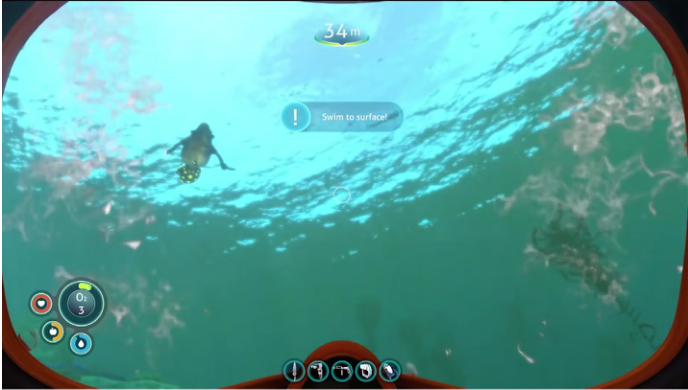
\includegraphics[width=0.72\linewidth]
      {../buku_ajar/chapters/15/figures/petunjuk-visual-dan-bunyi.png}\par
    \sumber{Peringatan disampaikan melalui tiga jalan sekaligus: angka, pesan
    tertulis, dan bunyi.}
  \end{column}
  \begin{column}{0.43\textwidth}
    \begin{itemize}
      \item Bunyi menjangkau pemain tanpa menuntut perhatian matanya, sehingga
            menjadi jalan kedua untuk menyampaikan keadaan permainan.
      \item Pada gambar, keadaan hampir kehabisan udara tampak pada angka,
            pesan tertulis, dan bunyi yang berubah mencekam.
      \item Setiap keterangan melalui bunyi sebaiknya disampaikan pula secara
            terlihat, agar tetap dipahami pemain yang pendengarannya terganggu.
    \end{itemize}
  \end{column}
\end{columns}
\vspace{0.10cm}
\begin{kotak}
Bunyi lompat berpasangan dengan animasi lompatan, bunyi mengambil benda dengan
skor yang bertambah, dan bunyi terluka dengan nyawa yang berkurang.
\end{kotak}
\end{frame}

\begin{frame}{Dua Jenis Bunyi: Musik Latar dan Efek Suara}
\awalan{Perbedaannya menentukan cara memuat, memutar, dan mengatur kekuatannya.}
{\scriptsize
\renewcommand{\arraystretch}{1.12}
\begin{tabularx}{\textwidth}{@{}>{\raggedright\arraybackslash}p{2.35cm}
    >{\raggedright\arraybackslash}p{5.55cm}
    >{\raggedright\arraybackslash}X@{}}
\toprule
\textbf{Segi} & \textbf{Musik latar (BGM)} & \textbf{Efek suara (SFX)} \\
\midrule
Lama berbunyi & Panjang, puluhan detik sampai beberapa menit &
  Pendek, umumnya di bawah dua detik \\
\addlinespace
Berapa kali & Satu berkas berjalan terus, diputar berulang &
  Banyak berkas pendek, dipanggil menurut kejadian \\
\addlinespace
Kapan dimulai & Ketika \emph{scene} dimuat, bukan ketika sesuatu terjadi &
  Ketika peristiwa permainan terjadi \\
\addlinespace
Boleh bertumpuk & Tidak; musik baru menimpa musik lama &
  Ya; dua bunyi dapat berbunyi bersamaan \\
\addlinespace
Letak di ruang & Di mana-mana; tidak berubah oleh posisi pemain &
  Umumnya pada tempat kejadian, ikut melemah menurut jarak \\
\addlinespace
Kekuatan & Lebih pelan, sebab berjalan terus-menerus &
  Lebih kuat, sebab harus terdengar di atas musik \\
\bottomrule
\end{tabularx}}
\vspace{0.14cm}
\begin{kotak}
Musik latar tidak boleh bertumpuk, sedangkan efek suara justru perlu dapat
bertumpuk. Pemain yang melompat sambil mengambil benda menimbulkan dua bunyi
dalam waktu yang sangat berdekatan.
\end{kotak}
\end{frame}

\begin{frame}{Jangan Memakai Satu Sumber untuk Keduanya}
\awalan{Kesalahan yang paling sering terjadi: satu \emph{AudioSource} dipakai
untuk musik dan efek suara sekaligus.}
\begin{itemize}
  \item Akibatnya, setiap efek suara menghentikan musik yang sedang berjalan;
        musik menjadi terputus-putus setiap pemain melompat atau mengambil
        benda.
  \item Pisahkan keduanya sejak awal, misalnya menjadi \texttt{musicSource}
        dan \texttt{sfxSource}, sebagaimana pada bab ini.
  \item Jenis bunyi ditentukan oleh keperluannya, bukan oleh berkasnya:
        pertanyaannya ``apakah bunyi ini berjalan terus, atau dipanggil menurut
        kejadian''.
\end{itemize}
\vspace{0.18cm}
\begin{peringatan}
Berkas yang sama dapat dipakai sebagai musik latar pada satu permainan dan
sebagai efek suara pada permainan lain. Yang membedakan bukan berkasnya,
melainkan cara ia dipanggil dan diperlakukan.
\end{peringatan}
\begin{kotak}
Satu sumber bunyi hanya memutar satu bunyi pada satu waktu. Itulah sebabnya
pemisahan sumber adalah syarat, bukan pilihan gaya.
\end{kotak}
\end{frame}

% ========================================================= bagian 2
\section{AudioClip, AudioSource, dan Ruang}
\sectionframe{02}{AudioClip, AudioSource, dan Ruang}
  {Berkasnya, pemutarnya, dan letaknya}

\begin{frame}{Dua Hal yang Berbeda}
\awalan{Pada Unity, bunyi dipisahkan menjadi dua hal: berkasnya dan pemutarnya.}
\begin{description}
  \item[\texttt{AudioClip}] Berkas bunyi yang telah diimpor, misalnya
        \texttt{lompat.wav}. Ia hanya berisi data: tidak tahu di mana ia
        berada, dan tidak dapat berbunyi sendiri.
  \item[\texttt{AudioSource}] Komponen yang menempel pada sebuah
        \emph{GameObject}. Ia yang memutar klip, mengatur kekuatannya, dan
        menentukan dari mana bunyinya terdengar.
\end{description}
\vspace{0.12cm}
\begin{itemize}
  \item \texttt{AudioClip} berperan seperti \emph{animation clip}: data yang
        tersimpan dan tidak berbuat apa-apa sendiri.
  \item \texttt{AudioSource} berperan seperti komponen \emph{Animator}:
        menempel pada benda dan mengurus pemutarannya.
  \item Karena itu, pertanyaan ``di mana bunyi ini terdengar'' selalu dijawab
        oleh letak \texttt{AudioSource}, bukan oleh berkasnya.
\end{itemize}
\begin{kotak}
Satu \texttt{AudioClip} dapat dipakai oleh beberapa \texttt{AudioSource},
misalnya bunyi langkah pada pemain dan pada NPC yang berbeda.
\end{kotak}
\end{frame}

\begin{frame}{Rantai Bunyi dari Peristiwa ke Pendengar}
\awalan{Kedua lajur---musik latar dan efek suara---bermuara pada satu titik.}
\centering
\adjustbox{max width=0.98\linewidth,max height=0.54\textheight}{%
  % chapters/15/figures/rantai-bunyi.tikz
% Jalan bunyi dari peristiwa permainan sampai ke pendengar.
\begin{tikzpicture}[
  tahap/.style={
    rectangle, rounded corners=5pt, draw=ubPrimary, thick, fill=ubAlt,
    align=center, text width=24mm, inner sep=3.5pt, minimum height=11mm,
    font=\footnotesize
  },
  sumber/.style={
    rectangle, rounded corners=5pt, draw=ubAccent, thick, fill=white,
    align=center, text width=24mm, inner sep=3.5pt, minimum height=11mm,
    font=\footnotesize
  },
  panah/.style={-{Stealth[length=2.2mm]}, thick, draw=ubAccent},
  catatan/.style={font=\scriptsize\itshape, align=left},
  judul/.style={font=\footnotesize\bfseries, ubPrimary}
]

\node[judul, anchor=west] at (-1.35,3.55) {Lajur BGM (musik latar)};
\node[judul, anchor=west] at (-1.35,-0.05) {Lajur SFX (efek suara)};

% --- Lajur BGM ---
\node[tahap]  (mulai) at (0,2.5)    {scene dimuat};
\node[tahap]  (putar) at (3.2,2.5)  {\code{PutarMusik()}};
\node[sumber] (srcA)  at (6.4,2.5)  {\code{AudioSource}\\{\scriptsize\itshape loop = true}};

% --- Lajur SFX ---
\node[tahap]  (kejadian) at (0,-1.0)   {peristiwa\\{\scriptsize\itshape lompat, ambil, terluka}};
\node[tahap]  (pemicu)   at (3.2,-1.0) {\code{PemicuBunyi}};
\node[sumber] (srcB)     at (6.4,-1.0) {\code{AudioSource}\\{\scriptsize\itshape PlayOneShot}};

% --- Titik temu ---
\node[sumber] (mix)    at (9.6,0.75) {\code{AudioMixer}\\{\scriptsize\itshape Musik dan Efek}};
\node[tahap]  (keluar) at (12.8,0.75) {pengeras suara};

\draw[panah] (mulai) -- (putar);
\draw[panah] (putar) -- (srcA);
\draw[panah] (srcA) -- (mix);
\draw[panah] (kejadian) -- (pemicu);
\draw[panah] (pemicu) -- (srcB);
\draw[panah] (srcB) -- (mix);
\draw[panah] (mix) -- (keluar);

\node[catatan, anchor=north west, text width=64mm] at (-1.35,-2.0)
  {Kedua lajur bertemu pada \istilah{AudioMixer}. Di sanalah perbandingan
   kekuatan musik dengan efek suara diatur, tanpa perlu mengubah berkas
   bunyinya.};
\end{tikzpicture}
}
\vspace{0.12cm}
\begin{kotak}
Kedua lajur bertemu pada \emph{AudioMixer}. Di sanalah perbandingan kekuatan
musik dengan efek suara diatur, tanpa perlu mengubah berkas bunyinya.
\end{kotak}
\end{frame}

\begin{frame}[fragile]{Pemusat Bunyi: Dua Sumber dan Lima Klip}
\lstinputlisting[language=CSharp,firstline=6,lastline=20]
  {../buku_ajar/code/unity/ch15_manajer_bunyi.cs}
\kodejelas{\texttt{Instance} dan \texttt{DontDestroyOnLoad} menjaga agar hanya
ada satu salinan yang hidup selama permainan, sehingga musik tidak terputus
ketika berpindah \emph{scene}. \texttt{musicSource} memutar BGM secara
berulang, \texttt{sfxSource} memainkan SFX sekali pakai, dan kelima klip
dihubungkan pada \emph{Inspector}.}
\end{frame}

\begin{frame}{Bunyi Datar, Bunyi Beruang, dan Dua Cara Memanggil}
\begin{columns}[T,onlytextwidth]
  \begin{column}{0.49\textwidth}
    \begin{block}{\emph{Spatial Blend}}
      \begin{itemize}
        \item Nilai nol: bunyi terdengar sama dari mana pun. Dipakai untuk
              musik latar dan seluruh bunyi antarmuka.
        \item Nilai satu: bunyi memiliki tempat dan melemah menurut jarak.
              Dipakai untuk bunyi benda di dalam level.
        \item \emph{Min Distance} menandai jarak bunyi mulai melemah;
              \emph{Max Distance} menandai jarak ia berhenti melemah.
        \item Nilai bawaan Unity sering terlalu besar untuk permainan dua
              dimensi.
      \end{itemize}
    \end{block}
  \end{column}
  \begin{column}{0.49\textwidth}
    \begin{block}{\texttt{Play} dan \texttt{PlayOneShot}}
      \begin{itemize}
        \item \texttt{PlayOneShot} dipakai untuk SFX: beberapa bunyi dapat
              berbunyi bersamaan pada satu sumber.
        \item Argumen keduanya menentukan kekuatan, misalnya
              \texttt{PlayOneShot(klipLompat, 0.8f)}.
        \item \texttt{Play} dipakai untuk musik latar: hanya satu musik yang
              boleh berjalan, dan musik lama memang harus berhenti.
      \end{itemize}
    \end{block}
  \end{column}
\end{columns}
\vspace{-0.06cm}
\begin{kotak}
Memanggil \texttt{PlayOneShot} tiga kali dalam tiga bingkai menghasilkan tiga
bunyi bertumpuk. Memakai \texttt{Play} dalam keadaan yang sama menghasilkan
satu bunyi yang selalu terpotong---terdengar seperti suara mesin yang patah.
\end{kotak}
\end{frame}

% ========================================================= bagian 3
\section{Memicu Bunyi dari Peristiwa Permainan}
\sectionframe{03}{Memicu Bunyi dari Peristiwa}
  {Daftar peristiwa, pemusatan skrip, dan pemicunya}

\begin{frame}{Daftar Peristiwa dan Bunyinya}
\awalan{Pekerjaan dimulai dari daftar, bukan dari kode. Sebagian peristiwa
datang dari \emph{trigger}, yaitu daerah yang tidak menghalangi gerak.}
{\scriptsize
\renewcommand{\arraystretch}{1.10}
\begin{tabularx}{\textwidth}{@{}>{\raggedright\arraybackslash}p{3.25cm}
    >{\raggedright\arraybackslash}p{2.55cm}
    >{\raggedright\arraybackslash}p{1.15cm}
    >{\raggedright\arraybackslash}X@{}}
\toprule
\textbf{Peristiwa} & \textbf{Bunyi} & \textbf{Jenis} & \textbf{Pasangan yang terlihat} \\
\midrule
\emph{Scene} dimulai & musik latar & BGM &
  Musik berjalan sejak layar pertama; tidak ada kekosongan sebelum pemain
  bergerak. \\
\addlinespace
Pemain melompat & \texttt{jumpSound} & SFX &
  Animasi lompatan, dan posisi pemain yang benar-benar naik. \\
\addlinespace
Pemain mengambil benda & \texttt{pickupSound} & SFX &
  Angka skor bertambah, dan bendanya menghilang. \\
\addlinespace
Pemain terluka & \texttt{hurtSound} & SFX &
  Jumlah nyawa berkurang, dan ikon nyawa ikut berubah. \\
\addlinespace
Pemain menyentuh tujuan & \texttt{winSound} & SFX &
  Pesan kemenangan, dan musik latar berhenti supaya tidak bersaing. \\
\addlinespace
Permainan berakhir & \texttt{gameOverSound} & SFX &
  Musik latar berhenti, lalu layar akhir muncul. \\
\bottomrule
\end{tabularx}}
\vspace{0.12cm}
\begin{kotak}
Kolom terakhir bukan hiasan: ia memaksa Anda memikirkan pasangan yang terlihat
bagi setiap bunyi. Bunyi tanpa pasangan yang terlihat perlu dipertanyakan.
\end{kotak}
\end{frame}

\begin{frame}[fragile]{Menghubungkan Lompat dan Pickup}
\lstinputlisting[language=CSharp,firstline=14,lastline=28]
  {../buku_ajar/code/unity/ch15_pemicu_bunyi.cs}
\kodejelas{Bunyi lompat dipanggil skrip kendali pemain (Bab XIII).
\texttt{CompareTag} membatasi bunyi dan skor pada benda bertanda \emph{pickup},
dan benda dimatikan agar sentuhan yang sama tidak terhitung dua kali.}
\end{frame}

\begin{frame}{Mengapa Bunyi Dipusatkan pada Satu Skrip}
\awalan{Pada Bab XIV setiap benda mengurus tampilannya sendiri. Untuk bunyi,
cara itu justru menyulitkan.}
\begin{enumerate}
  \item Ada dua hal yang harus berlaku bagi seluruh permainan sekaligus: hanya
        satu musik yang boleh berjalan, dan perbandingan kekuatan musik dengan
        efek suara harus tetap sama.
  \item Karena itu, setiap bagian permainan memanggil skrip pemusat, dan tidak
        memainkan bunyinya sendiri-sendiri.
  \item Susunan itu tampak pada rantai bunyi: seluruh lajur bermuara pada satu
        titik, yaitu \texttt{ManajerBunyi}.
  \item Rujukan yang belum dihubungkan pada \emph{Inspector} bernilai kosong;
        pemeriksaan \texttt{if (manajer != null)} membuat kesalahan pemasangan
        mudah ditemukan, bukan kegagalan yang membingungkan.
\end{enumerate}
\vspace{0.12cm}
\begin{kotak}
Kebiasaan memeriksa sebelum memanggil dipakai berulang-ulang pada skrip bab
ini. Ia bukan kelebihan, melainkan cara agar permainan tidak berhenti dengan
kesalahan.
\end{kotak}
\end{frame}

\begin{frame}[fragile]{Peristiwa Terluka dan Kalah}
\lstinputlisting[language=CSharp,firstline=32,lastline=41]
  {../buku_ajar/code/unity/ch15_pemicu_bunyi.cs}
\kodejelas{Kedua fungsi meneruskan peristiwa tabrakan dan kalah kepada pemusat;
skrip pemicu tidak menyimpan bunyi sendiri.}
\begin{itemize}
  \item \texttt{Terluka} memanggil bunyi terluka sekaligus mengurangi nyawa
        pada antarmuka, sehingga bunyi dan pasangan terlihatnya berjalan
        bersama.
  \item \texttt{Kalah} menghentikan musik latar lebih dahulu, lalu memutar
        \texttt{gameOverSound}, supaya keduanya tidak bersaing.
\end{itemize}
\end{frame}

% ========================================================= bagian 4
\section{Waktu dan Kekuatan Bunyi}
\sectionframe{04}{Waktu dan Kekuatan Bunyi}
  {Kapan dipanggil, seberapa kuat, dan mengapa desibel}

\begin{frame}{Tingkat Kekuatan Bunyi pada AudioMixer}
\awalan{Susunan tingkat kekuatan yang dipakai pada bab ini.}
\centering
\adjustbox{max width=0.92\linewidth,max height=0.50\textheight,scale=1.08}{%
  % chapters/15/figures/hierarki-volume.tikz
% Susunan tingkat kekuatan bunyi: satu induk, dua cabang, dan nilai yang
% biasanya dipakai pada setiap tingkat.
\begin{tikzpicture}[
  tingkat/.style={
    rectangle, rounded corners=5pt, draw=ubPrimary, thick, fill=ubAlt,
    align=center, text width=26mm, inner sep=4pt, minimum height=11mm,
    font=\footnotesize
  },
  panah/.style={-{Stealth[length=2.2mm]}, thick, draw=ubAccent},
  nilai/.style={font=\scriptsize, ubPrimary},
  catatan/.style={font=\scriptsize\itshape, align=left}
]

\node[tingkat] (master) at (3.5,1.5) {\code{Master}\\{\scriptsize\itshape seluruh bunyi}};
\node[tingkat] (musik)  at (0.6,-0.9) {\code{Musik}\\{\scriptsize\itshape BGM}};
\node[tingkat] (efek)   at (6.4,-0.9) {\code{Efek}\\{\scriptsize\itshape SFX}};

\draw[panah] (master) -- (musik);
\draw[panah] (master) -- (efek);

\node[nilai, right=1pt] at (master.east) {0 dB};
\node[nilai, below=0.5pt] at (musik.south) {$-12$ dB};
\node[nilai, below=0.5pt] at (efek.south) {$-6$ dB};

\node[catatan, anchor=north west, text width=78mm] at (-0.9,-2.2)
  {Angka pada \istilah{AudioMixer} memakai satuan desibel, yang naik secara
   berlipat, bukan secara lurus. Menurunkan 6 dB berarti mengurangi
   kekuatannya menjadi kira-kira separuh. Karena itu, penggeser pada menu
   pengaturan sebaiknya tetap bernilai lurus dari 0 sampai 1, lalu diubah ke
   desibel melalui perhitungan.};
\end{tikzpicture}
}
\vspace{0.10cm}
\begin{itemize}
  \item \texttt{Master} pada 0 dB, \texttt{Musik} pada $-12$ dB, dan
        \texttt{Efek} pada $-6$ dB.
  \item Angka itu titik awal, bukan patokan: yang menentukan adalah pendengaran
        Anda pada level Anda sendiri.
  \item Mata rantai yang paling sering salah adalah efek suara yang terlalu
        pelan, bukan yang terlalu kuat.
\end{itemize}
\end{frame}

\begin{frame}{Bunyi Dipanggil pada Peristiwanya}
\awalan{Indikator ketiga menuntut lebih dari sekadar ``bunyi sudah terpasang'':
bunyi harus terdengar pada saat yang tepat.}
\begin{enumerate}
  \item \textbf{Pada peristiwa, bukan pada keadaan.} Bunyi lompat dipanggil
        ketika tombol ditekan, bukan selama tombol tertahan. Memanggilnya
        berdasarkan keadaan menghasilkan bunyi berulang setiap bingkai.
  \item \textbf{Perhatikan di mana pemeriksaan dilakukan.} Bunyi tidak
        berkaitan dengan fisika, sehingga dipanggil di \texttt{Update}, bukan
        di \texttt{FixedUpdate}.
  \item \textbf{Jangan menunggu animasi selesai.} Bunyi adalah umpan balik
        seketika; menundanya sampai animasi mencapai bingkai tertentu membuat
        permainan terasa lamban.
\end{enumerate}
\vspace{0.14cm}
\begin{peringatan}
Bingkai fisika berjalan lebih jarang daripada bingkai tampilan. Bunyi yang baru
dipanggil di \texttt{FixedUpdate} dapat tertunda dua sampai tiga bingkai; pada
60 bingkai per detik itu sekitar 50 milidetik, dan pada bunyi pendek penundaan
sebesar itu sudah terasa.
\end{peringatan}
\end{frame}

\begin{frame}{Mengapa Satuannya Desibel}
\awalan{Kekuatan bunyi pada \emph{AudioMixer} dinyatakan dalam desibel, dan
satuannya tidak naik secara lurus.}
\begin{itemize}
  \item Menurunkan 6 dB berarti mengurangi kekuatannya menjadi kira-kira
        separuh; menaikkan 6 dB berarti melipatgandakannya.
  \item Penggeser pada menu pengaturan sebaiknya tetap bernilai lurus dari nol
        sampai satu, lalu diubah ke desibel sebelum diberikan kepada
        \emph{AudioMixer}.
  \item Nilai nol tidak dapat diubah, sebab desibelnya menuju tak hingga
        negatif; nilai $-80$ dB dipakai sebagai pengganti senyap.
\end{itemize}
\[
L = 20\,\log_{10}(v)
\qquad\text{misalnya } v = 0{,}5 \;\Rightarrow\; L \approx -6\ \text{dB}.
\]
\begin{kotak}
Selisih sekitar 10 dB antara efek suara dan musik latar adalah titik awal yang
baik. Menyeimbangkan bunyi lebih sering berarti menurunkan yang terlalu kuat
daripada menaikkan yang terlalu pelan.
\end{kotak}
\end{frame}

\begin{frame}[fragile]{Menggeser Nada agar Tidak Seperti Mesin}
\lstinputlisting[language=CSharp,firstline=66,lastline=76]
  {../buku_ajar/code/unity/ch15_manajer_bunyi.cs}
\kodejelas{Nada digeser antara 0,92 dan 1,08 kali nada aslinya, dengan besar yang
berbeda-beda setiap panggilan.}
\begin{itemize}
  \item Nilai delapan persen dipakai pada bab ini. Lebih dari itu bunyi mulai
        terdengar berubah-ubah seperti mainan; kurang dari itu pengulangannya
        masih terdengar.
  \item \texttt{PlayOneShot} menerima kekuatan bunyi sebagai argumen kedua,
        sehingga satu berkas dapat dipakai untuk beberapa keperluan.
\end{itemize}
\end{frame}

\begin{frame}{Empat Percobaan yang Perlu Dilakukan}
\awalan{Nilai pada bab ini adalah titik awal. Setiap percobaan cukup dilakukan
dengan mengubah satu nilai lalu menjalankan kembali permainannya.}
{\scriptsize
\renewcommand{\arraystretch}{1.12}
\begin{tabularx}{\textwidth}{@{}>{\raggedright\arraybackslash}p{3.55cm}
    >{\raggedright\arraybackslash}p{3.35cm}
    >{\raggedright\arraybackslash}X@{}}
\toprule
\textbf{Yang diubah} & \textbf{Menjadi} & \textbf{Yang akan Anda dengar} \\
\midrule
\texttt{musicVolume} & 0,2 lalu 1,0 &
  Pada nilai rendah efek suara mendominasi; pada nilai tinggi bunyi lompat
  mulai tertelan musik. \\
\addlinespace
\texttt{pitchVariation} & 0,0 lalu 0,25 &
  Pada nilai nol bunyi berulang terdengar seperti mesin; pada nilai terlalu
  besar bunyinya berubah-ubah seperti mainan. \\
\addlinespace
\texttt{PlayOneShot} diganti \texttt{Play} & Pada skrip langkah &
  Dua langkah yang berdekatan saling memotong, sehingga bunyinya
  terputus-putus. \\
\addlinespace
\emph{Spatial Blend} pada bunyi benda & 0 lalu 1 &
  Pada nilai nol, bunyi benda di sudut level terdengar sama kuatnya dengan yang
  ada di dekat pemain. \\
\bottomrule
\end{tabularx}}
\vspace{0.14cm}
\begin{kotak}
Mengubah satu nilai lalu mendengarkan akibatnya adalah cara satu-satunya untuk
memahami tingkat kekuatan bunyi. Catat hasil setiap percobaan, sebelum dan
sesudah nilainya diubah.
\end{kotak}
\end{frame}

% ========================================================= bagian 5
\section{Partikel Sederhana}
\sectionframe{05}{Partikel Sederhana}
  {Pasangan yang terlihat bagi peristiwa sekejap}

\begin{frame}{Partikel: Pasangan yang Terlihat untuk Peristiwa Sekejap}
\awalan{\emph{Partikel} adalah kumpulan gambar kecil yang muncul, bergerak,
lalu menghilang. Satu ledakan kecil, satu kepulan debu, atau satu kilau ketika
benda diambil.}
\begin{description}
  \item[\emph{Duration} dan \emph{Looping}] Lama satu putaran partikel dan
        apakah ia diulang. Untuk bunyi yang dipicu peristiwa, \emph{Looping}
        dimatikan sebab partikelnya diputar sekali saja.
  \item[\emph{Start Lifetime}] Lama setiap partikel hidup sebelum hilang.
        Untuk percikan kecil, seperlima sampai setengah detik sudah cukup.
  \item[\emph{Start Speed}] Kecepatan awal partikel meninggalkan pusatnya.
        Nilai besar memberi kesan ledakan; nilai kecil memberi kesan kepulan.
  \item[\emph{Emission} dan \emph{Bursts}] Jumlah partikel per satuan waktu.
        \emph{Bursts} mengeluarkan sekumpulan partikel sekaligus pada satu
        saat, dan itulah yang sesuai untuk peristiwa sekejap.
\end{description}
\vspace{0.10cm}
\begin{peringatan}
Jangan memakai partikel untuk menutupi masalah. Apabila sebuah mekanik tidak
terasa jelas tanpa partikel, kemungkinan besar mekaniknya sendiri belum jelas.
\end{peringatan}
\end{frame}

\begin{frame}[fragile]{Memanggil Partikel pada Peristiwa yang Sama}
\awalan{Partikel dipanggil pada peristiwa yang sama dengan bunyinya, sehingga
keduanya muncul bersamaan.}
\begin{lstlisting}
// Ditambahkan pada PemicuBunyi, disimpan pada peubah partikel.
public ParticleSystem partikelAmbil;

void OnTriggerEnter2D(Collider2D lain)
{
    if (!lain.CompareTag("Pickup")) return;

    if (manajer != null) manajer.BunyiAmbil();
    if (partikelAmbil != null) partikelAmbil.Play();
    ...
}
\end{lstlisting}
\kodejelas{\texttt{ParticleSystem.Play()} dipanggil di tempat yang sama persis
dengan bunyinya. Itu bukan kebetulan: keduanya tanggapan atas satu peristiwa,
dan keduanya sebaiknya diurus pada satu tempat agar tidak ada yang tertinggal.}
\end{frame}

% ========================================================= bagian 6
\section{Pygame, Unity, dan Hak Pakai Bunyi}
\sectionframe{06}{Pygame, Unity, dan Hak Pakai Bunyi}
  {Perbandingan, lisensi, dan penutup bab}

\begin{frame}{Cara yang Sudah Anda Pakai: Pygame dan Unity}
\awalan{Pemisahan bunyi di Pygame bukan kebetulan, melainkan kebutuhan yang sama
yang Anda temui kembali pada Unity.}
{\scriptsize
\renewcommand{\arraystretch}{1.12}
\begin{tabularx}{\textwidth}{@{}>{\raggedright\arraybackslash}p{3.2cm}
    >{\raggedright\arraybackslash}p{4.9cm}
    >{\raggedright\arraybackslash}X@{}}
\toprule
\textbf{Keperluan} & \textbf{Pygame} & \textbf{Unity} \\
\midrule
Memuat berkas bunyi & \texttt{mixer.Sound("a.wav")} &
  Diimpor seperti gambar, lalu diseret ke peubah \texttt{AudioClip} pada
  \emph{Inspector}. \\
\addlinespace
Memainkan efek suara & \texttt{bunyi.play()} &
  \texttt{sfxSource.PlayOneShot(klip)}. \\
\addlinespace
Memutar musik berulang & \texttt{mixer.music.load()} lalu
  \texttt{mixer.music.play(-1)} &
  \texttt{musicSource.loop = true} lalu \texttt{musicSource.Play()}. \\
\addlinespace
Mengatur kekuatan & \texttt{bunyi.set\_volume(0.5)} &
  Nilai pada \emph{AudioSource}, atau tingkat pada \emph{AudioMixer}. \\
\addlinespace
Melemahkan menurut jarak & Harus dihitung sendiri dari jarak pemain &
  Diurus mesin melalui \emph{Spatial Blend} dan \emph{Min Distance}. \\
\bottomrule
\end{tabularx}}
\vspace{0.14cm}
\begin{kotak}
Satu pelajaran dari Pygame tetap berlaku: sediakan jalan bagi pemain untuk
mematikan bunyinya. Pemain yang bermain di tempat ramai akan berterima kasih
untuk pilihan itu.
\end{kotak}
\end{frame}

\begin{frame}{Hak Pakai Berkas Bunyi}
\awalan{Aturan pada Bab XIV berlaku sama untuk bunyi, dan akibatnya justru
lebih berat.}
\begin{itemize}
  \item Berkas musik lebih mudah dikenali daripada gambar, penuntutan hak
        ciptanya lebih lazim, dan satu potongan tanpa izin dapat membatalkan
        seluruh proyek.
  \item Cari tempat yang menyatakan lisensinya dengan jelas; situs musik bebas
        biasanya mencantumkan jenis lisensi pada setiap berkas.
  \item Catat sejak mengunduh: nama berkas, sumber, jenis lisensi, dan apakah
        penciptanya menuntut namanya dicantumkan.
  \item Pisahkan musik untuk keperluan belajar dari musik untuk karya yang
        dijual; sebagian lisensi mengizinkan yang pertama, tidak yang kedua.
\end{itemize}
\vspace{0.16cm}
\begin{kiat}
Bunyi juga dapat dibuat sendiri, dan untuk mata kuliah ini cara itu sering lebih
cepat daripada mencari. Sebuah bunyi lompat dapat dibuat dari satu bunyi pendek
yang nadanya dinaikkan sedikit.
\end{kiat}
\end{frame}

% --------------------------------------------------------- aktivitas
\begin{frame}{Aktivitas di Kelas \textperiodcentered\ Praktikum 12}
\setbeamerfont{itemize/enumerate body}{size=\scriptsize}
\awalan{Pengalaman belajar minggu 14 pada RPS, dikerjakan berurutan di kelas lalu
diselesaikan di rumah.}
\begin{enumerate}
  \item Kumpulkan satu berkas musik latar dan sekurang-kurangnya empat efek
        suara: lompat, mengambil benda, terluka, dan kalah. Catat sumber serta
        lisensi setiap berkas sejak awal.
  \item Impor berkasnya, atur \emph{Load In Background} pada musik dan
        \emph{Decompress On Load} pada efek suara pendek.
  \item Buat \emph{GameObject} \texttt{ManajerBunyi} dengan dua
        \texttt{AudioSource}---\texttt{musicSource} dan \texttt{sfxSource}---lalu
        tempel \texttt{ch15\_manajer\_bunyi.cs} dan hubungkan keenam rujukannya.
  \item Atur \emph{Spatial Blend} nol pada musik dan efek suara pemain; tempel
        \texttt{ch15\_pemicu\_bunyi.cs} pada pemain; tambahkan dua baris pada
        \texttt{ch13\_kontrol\_pemain.cs}; tandai benda dengan \emph{Tag}
        \texttt{Pickup}.
  \item Susun \emph{AudioMixer} dengan tingkat \texttt{Master}, \texttt{Musik},
        dan \texttt{Efek}, lalu jalankan keempat percobaan dan catat hasilnya.
  \item Tambahkan satu partikel sederhana pada satu peristiwa, tulis catatan
        praktikum, lalu simpan ke repositori Git.
\end{enumerate}
\vspace{0.08cm}
{\footnotesize\color{ubAccent}\itshape Rincian lengkap: Praktikum 12 pada
Bab XV buku ajar. Kumpulkan melalui repositori Git pribadi.}
\end{frame}

% --------------------------------------------------------- rangkuman
\begin{frame}{Rangkuman}
\begin{itemize}
  \item Bunyi menjangkau pemain tanpa menuntut perhatian matanya; karena itu
        setiap bunyi sebaiknya memiliki pasangan yang terlihat.
  \item Musik latar berjalan terus dan tidak boleh bertumpuk; efek suara
        dipanggil menurut kejadian dan justru perlu dapat bertumpuk.
  \item \texttt{AudioClip} adalah datanya, \texttt{AudioSource} adalah
        pemutarnya; letak bunyi ditentukan oleh sumber, bukan oleh berkasnya.
  \item Bunyi dipusatkan pada satu skrip: \texttt{PlayOneShot} untuk efek suara,
        \texttt{Play} untuk musik latar.
  \item Bunyi dipanggil pada peristiwa di \texttt{Update}; kekuatan dinyatakan
        dalam desibel, dan selisih sekitar 10 dB adalah titik awal yang baik.
  \item Partikel adalah pasangan yang terlihat bagi bunyi dan dipanggil pada
        peristiwa yang sama; sumber serta lisensi berkas bunyi wajib dicatat.
\end{itemize}
\end{frame}

% --------------------------------------------------------- cek
\begin{frame}{Cek Pemahaman}
\begin{enumerate}
  \item Mengapa satu \texttt{AudioSource} tidak boleh dipakai untuk musik dan
        efek suara sekaligus, dan gejala apa yang muncul?
  \item Mengapa bunyi dipanggil di \texttt{Update}, bukan di
        \texttt{FixedUpdate}?
  \item Musik bernilai $-6$ dB dan efek suara bernilai $-6$ dB. Mengapa bunyi
        lompatan tetap terdengar samar, dan apa yang sebaiknya diubah?
\end{enumerate}
\vspace{0.35cm}
{\footnotesize\color{ubMuted}\itshape Jawab tanpa membuka catatan, lalu
bandingkan dengan pasangan di sebelah Anda.}
\end{frame}

% --------------------------------------------------------- penutup
\penutup{Tugas Praktikum 12}
  {Materi 14 \textperiodcentered\ Evaluasi Prototipe, \emph{Playtesting}, dan
   Presentasi: bunyi dan partikel yang baru dipasang diuji oleh pemain lain
   pada \emph{playtest}, lalu demo proyek akhir ditampilkan. Ketidakcocokan
   \emph{timing} dan kekuatan bunyi akan muncul di sana.}

\end{document}
